% !TeX spellcheck = sl_SI
% vim: set spell spelllang=sl:
% za preverjanje črkovanja, če se uporablja Texstudio ali vim
\documentclass[12pt,a4paper,twoside]{article}
\usepackage[utf8]{inputenc}  % pravilno razpoznavanje unicode znakov

% NASLEDNJE UKAZE USTREZNO POPRAVI
\newcommand{\program}{Matematika} % ime studijskega programa
\newcommand{\imeavtorja}{Ines Meršak} % ime avtorja
\newcommand{\imementorja}{prof.~dr.~Sandi Klavžar} % akademski naziv in ime mentorja, uporabi poln naziv, prof.~dr.~, doc.~dr., ali izr.~prof.~dr.
\newcommand{\imesomentorja}{} % akademski naziv in ime somentorja, če ga imate
\newcommand{\naslovdela}{Ničelna prisila}
\newcommand{\letnica}{2019} % letnica magistriranja
\newcommand{\opis}{Delo obravnava integracijo po ω-kompleksih, njene lastnosti in posplošitve
na Levy-jeve topološke prostore.}  % Opis dela v eni povedi. Ne sme vsebovati matematičnih simbolov v $ $.
\newcommand{\kljucnebesede}{integracija\sep kompleks} % ključne besede, ločene z \sep, da se PDF metapodatki prav procesirajo
\newcommand{\keywords}{integration\sep complex} % ključne besede v angleščini
\newcommand{\organization}{Univerza v Ljubljani, Fakulteta za matematiko in fiziko} % fakulteta
\newcommand{\literatura}{literatura}  % pot do datoteke z literaturo (brez .bib končnice)
\newcommand{\sep}{, }  % separator med ključnimi besedami v besedilu
% KONEC PODATKOV

\usepackage{bibentry}         % za navajanje literature v programu dela s celim imenom
\nobibliography{\literatura}
\newcommand{\plancite}[1]{\item[\cite{#1}] \bibentry{#1}} % citiranje v programu dela

\usepackage{filecontents}  % za pisanje datoteke s PDF metapodatki
\usepackage{silence} \WarningFilter{latex}{Overwriting file}  % odstrani annoying warning o obstoju datoteke
% datoteka s PDF metapodatki, zgenerira se kot magisterij.xmpdata
\begin{filecontents*}{\jobname.xmpdata}
  \Title{\naslovdela}
  \Author{\imeavtorja}
  \Keywords{\kljucnebesede}
  \Subject{matematika}
  \Org{\organization}
\end{filecontents*}

\usepackage[a-1b]{pdfx}  % zgenerira PDF v tem PDF/A-1b formatu, kot zahteva knjižnica
\hypersetup{bookmarksopen, bookmarksdepth=3, colorlinks=true,
  linkcolor=black, anchorcolor=black, citecolor=black, filecolor=black,
  menucolor=black, runcolor=black, urlcolor=black, pdfencoding=auto,
  breaklinks=true, psdextra}

\usepackage[slovene]{babel}  % slovenščina
\usepackage[T1]{fontenc}     % naprednejše kodiranje fonta
\usepackage{amsmath,amssymb,amsfonts,amsthm} % matematični paketi
\usepackage[dvipsnames,usenames]{color} % barve
\usepackage{graphicx}     % za slike
\usepackage{emptypage}    % prazne strani so neoštevilčene, ampak so štete
\usepackage{units}        % fizikalne enote kot \unit[12]{kg} s polovico nedeljivega presledka, glej primer v kodi
%\usepackage{makeidx}      % za stvarno kazalo, lahko zakomentiraš, če ne rabiš
%\makeindex                % za stvarno kazalo, lahko zakomentiraš, če ne rabiš
% oblika strani
\usepackage[
  top=3cm,
  bottom=3cm,
  inner=3.5cm,      % margini za dvostransko tiskanje
  outer=2.5cm,
  footskip=40pt     % pozicija številke strani
]{geometry}

% VEČ ZANIMIVIH PAKETOV
% \usepackage{array}      % več možnosti za tabele
 \usepackage[list=true,listformat=simple]{subcaption}  % več kot ena slika na figure, omogoči slika 1a, slika 1b
% \usepackage[all]{xy}    % diagrami
% \usepackage{doi}        % za clickable DOI entrye v bibliografiji
% \usepackage{enumerate}     % več možnosti za sezname

% Za barvanje source kode
% \usepackage{minted}
% \renewcommand\listingscaption{Program}

% Za pisanje psevdokode
% \usepackage{algpseudocode}  % za psevdokodo
% \usepackage{algorithm}
% \floatname{algorithm}{Algoritem}
% \renewcommand{\listalgorithmname}{Kazalo algoritmov}

% DRUGI TVOJI PAKETI:
\usepackage[labelfont=it, format=hang]{caption}
\usepackage{tikz}
\usetikzlibrary{math}
\usepackage{mathtools}

\setlength{\overfullrule}{50pt} % označi predlogo vrstico
\pagestyle{plain}               % samo številka strani na dnu, nobene glave / noge

% ukazi za matematična okolja
\theoremstyle{definition} % tekst napisan pokončno
\newtheorem{definicija}{Definicija}[section]
\newtheorem{primer}[definicija]{Primer}
\newtheorem{opomba}[definicija]{Opomba}
\newtheorem{aksiom}{Aksiom}

\theoremstyle{plain} % tekst napisan poševno
\newtheorem{lema}[definicija]{Lema}
\newtheorem{izrek}[definicija]{Izrek}
\newtheorem{trditev}[definicija]{Trditev}
\newtheorem{posledica}[definicija]{Posledica}

\numberwithin{equation}{section}  % števec za enačbe zgleda kot (2.7) in se resetira v vsakem poglavju

% Matematični ukazi
\newcommand{\R}{\mathbb R}
\newcommand{\N}{\mathbb N}
\newcommand{\Z}{\mathbb Z}
\renewcommand{\C}{\mathbb C}
\newcommand{\Q}{\mathbb Q}
\newcommand{\F}{\mathbb F}
\renewcommand{\G}{\mathcal{G}}

\DeclareMathOperator{\boxempty}{\Box}

% bold matematika znotraj \textbf{ }, tudi v naslovih, kot \omega spodaj
\makeatletter \g@addto@macro\bfseries{\boldmath} \makeatother

% Poimenuj kazalo slik kot ``Kazalo slik'' in ne ``Slike''
\addto\captionsslovene{
  \renewcommand{\listfigurename}{Kazalo slik}%
}

% če želiš, da se poglavja začnejo na lihih straneh zgoraj
% \let\oldsection\section
% \def\section{\cleardoublepage\oldsection}

%%%%%%%%%%%%%%%%%%%%%%%%%%%%%%%%%%%%%%%%%%
%%%%%%           DOCUMENT           %%%%%%
%%%%%%%%%%%%%%%%%%%%%%%%%%%%%%%%%%%%%%%%%%

\begin{document}

\pagenumbering{roman} % začnemo z rimskimi številkami
\thispagestyle{empty} % ampak na prvi strani ni številke

\noindent{\large
UNIVERZA V LJUBLJANI\\[1mm]
FAKULTETA ZA MATEMATIKO IN FIZIKO\\[5mm]
\program\ -- 2.~stopnja}
% ustrezno dopolni za IŠRM
\vfill

\begin{center}
  \large
  \imeavtorja\\[3mm]
  \Large
  \textbf{\MakeUppercase{\naslovdela}}\\[10mm]
  \large
  Magistrsko delo \\[1cm]
  Mentor: \imementorja \\[2mm] % ustrezno popravi spol
%   Somentor: \imesomentorja   % dodaj, če potrebno
\end{center}
\vfill

\noindent{\large Ljubljana, \letnica}

\cleardoublepage

%% sem pride IZJAVA O AVTORSTVU  -- SE NATISNE V VIS

% zahvala
\pdfbookmark[1]{Zahvala}{zahvala} %
\section*{Zahvala}
Neobvezno.
Zahvaljujem se \dots
% end zahvala -- izbriši vse med zahvala in end zahvala, če je ne rabiš

\cleardoublepage

\pdfbookmark[1]{\contentsname}{kazalo-vsebine}
\tableofcontents

% list of figures
% \cleardoublepage
% \pdfbookmark[1]{\listfigurename}{kazalo-slik}
% \listoffigures
% end list of figures

\cleardoublepage

\section*{Program dela}
\addcontentsline{toc}{section}{Program dela} % dodajmo v kazalo
Mentor naj napiše program dela skupaj z osnovno literaturo. Na literaturo se
lahko sklicuje kot~\cite{lebedev2009introduction}, \cite{gurtin1982introduction},
\cite{zienkiewicz2000finite}, \cite{STtemplate}.

\section*{Osnovna literatura}
Literatura mora biti tukaj posebej samostojno navedena (po pomembnosti) in ne
le citirana. V tem razdelku literature ne oštevilčimo po svoje, ampak uporabljamo
okolje itemize in ukaz plancite, saj je celotna literatura oštevilčena na koncu.
\begin{itemize}
  \plancite{lebedev2009introduction}
  \plancite{gurtin1982introduction}
  \plancite{zienkiewicz2000finite}
  \plancite{STtemplate}
\end{itemize}

\vspace{2cm}
\hspace*{\fill} Podpis mentorja: \phantom{prostor za podpis}

% \vspace{2cm}
% \hspace*{\fill} Podpis somentorja: \phantom{prostor za podpis}

\cleardoublepage
\pdfbookmark[1]{Povzetek}{abstract}

\begin{center}
\textbf{\naslovdela} \\[3mm]
\textsc{Povzetek} \\[2mm]
\end{center}
Tukaj napišemo povzetek vsebine. Sem sodi razlaga vsebine in ne opis tega, kako je delo
organizirano.

\vfill
\begin{center}
\textbf{English translation of the title} \\[3mm] % prevod slovenskega naslova dela
\textsc{Abstract}\\[2mm]
\end{center}

An abstract of the work is written here. This includes a short description of
the content and not the structure of your work.

\vfill\noindent
\textbf{Math.~Subj.~Class.~(2010):} oznake kot 74B05, 65N99, na voljo so na naslovu
\url{http://www.ams.org/msc/msc2010.html?t=65Mxx} \\[1mm]
\textbf{Ključne besede:} \kljucnebesede \\[1mm]
\textbf{Keywords:} \keywords

\cleardoublepage

\setcounter{page}{1}    % od sedaj naprej začni zopet z 1
\pagenumbering{arabic}  % in z arabskimi številkami

\section{Uvod}
Napišite kratek zgodovinski in matematični uvod.  Pojasnite motivacijo za problem, kje
nastopa, kje vse je bil obravnavan. Na koncu opišite tudi organizacijo dela -- kaj je v kakšnem
razdelku.

\section{Osnovne definicije}
V tem poglavju najprej navedemo nekaj osnovnih definicij teorije grafov, nato pa definiramo dva temeljna pojma tega dela, množico ničelne prisile in število ničelne prisile, si ogledamo motivacijo za poimenovanje in nekaj primerov.

\emph{Graf} $G$ je definiran kot urejen par množice vozlišč, označimo jih z $V(G)$, in množice povezav $E(G)$, pri čemer so povezave pari elementov iz $V(G)$. Za potrebe tega dela bo za graf veljalo, da je končen (dovolj je, če je končna množica vozlišč) in ima neprazno množico vozlišč, nima zank (nobena povezava ne sme biti sestavljena samo iz enega vozlišča) in večkratnih povezav (elementi v $E(G)$ se ne ponavljajo). Če so elementi množice povezav urejeni pari, pravimo, da je graf \emph{usmerjen}, v nasprotnem primeru pa \emph{neusmerjen}. Če ni označeno drugače, bomo z besedo graf mislili neusmerjen povezan graf. \emph{Velikost grafa} $G$ je definirano kot število vozlišč tega grafa, označimo tudi kot $|G|$. V nadaljevanju bomo, kjer je očitno, za kateri graf gre, množico vozlišč grafa označevali kar z $V$, množico povezav pa z $E$. 

Vozlišči $u$ in $v$ sta \emph{sosednji}, če obstaja povezava med njima, torej $\{u,v\} \in E$, pišemo tudi $u \sim_G v$ ali kar $u \sim v$. (Pri pisanju povezav bomo ponavadi izpuščali oklepaje in vejico, namesto $\{u,v\}$ torej pišimo kar $uv$.) \emph{Soseščina vozlišča} $u$ je množica tistih vozlišč, ki so mu sosednja, \emph{stopnja vozlišča} v grafu $G$ pa je število njegovih sosedov. Največjo stopnjo nekega vozlišča v grafu $G$ bomo označili z $\Delta(G)$, najmanjšo pa z $\delta(G)$. Kadar je očitno, za kateri graf gre, bomo pisali kar $\Delta$ in $\delta$.

\subsection{Produkti grafov}
V delu si bomo ogledali tudi rezultate za nekatere produkte grafov, zato jih najprej definirajmo in ilustrirajmo s primeri.

\begin{definicija}
    \emph{Kartezični produkt} grafov $G$ in $H$, označimo $G \boxempty H$, je graf, katerega  množica vozlišč je kartezični produkt množice vozlišč grafa $G$ in grafa $H$, sosednji pa sta tisti dve vozlišči $(u, v)$ in $(u', v')$, $u, u' \in V(G),\ v, v' \in V(H)$, za kateri velja eden izmed naslednjih pogojev:
    \begin{enumerate}
        \item $u = u'$ in $vv' \in E(H)$,
        \item $v = v'$ in $uu' \in E(G)$.
    \end{enumerate}
\end{definicija}

\begin{definicija}
    \emph{Krepki produkt} grafov $G$ in $H$, označimo $G \boxtimes H$, je graf, katerega  množica vozlišč je kartezični produkt množice vozlišč grafa $G$ in grafa $H$, sosednji pa sta tisti dve vozlišči $(u, v)$ in $(u', v')$, $u, u' \in V(G),\ v, v' \in V(H)$, za kateri velja eden izmed naslednjih pogojev:
    \begin{enumerate}
        \item $u = u'$ in $vv' \in E(H)$,
        \item $v = v'$ in $uu' \in E(G)$,
        \item $uu' \in E(G)$ in $vv' \in E(H)$.
    \end{enumerate}
\end{definicija}

Iz definicij opazimo, da velja $E(G \boxempty H) \subseteq E(G \boxtimes H)$. Poglejmo si  nekaj primerov obeh produktov z enostavnimi družinami grafov.

\begin{primer}
    Najprej si poglejmo primera kartezičnega produkta poti $P_2 \boxempty P_3$ in krepkega produkta poti $P_2 \boxtimes P_3$, ki sta prikazana na sliki~\ref{fig:produkta-poti}.
    \begin{figure}[h]
        \begin{subfigure}{0.5\textwidth}
            \centering
            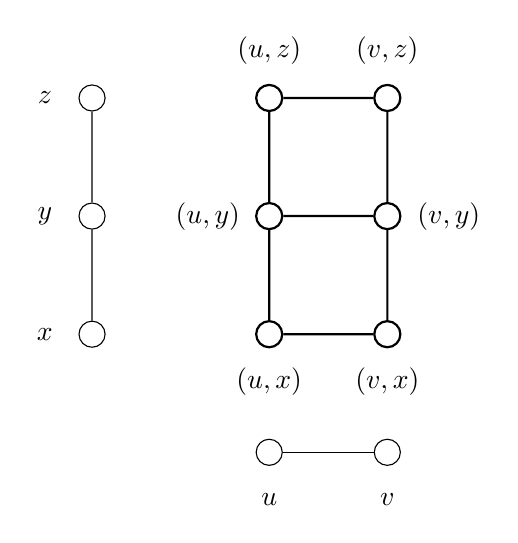
\begin{tikzpicture}[xscale=1.5, yscale=1.5]
                \tikzmath{\o = 0.4;}
                \begin{scope}[every node/.style={circle,draw}]
                \node (u) at (1,0) {};
                \node (v) at (2,0) {};
                
                \node (x) at (-0.5,1) {};
                \node (y) at (-0.5,2) {};
                \node (z) at (-0.5,3) {};
                \end{scope}
                
                \node at (1, -\o) {$u$};
                \node at (2, -\o) {$v$};
                
                \node at (-0.5-\o, 1) {$x$};
                \node at (-0.5-\o, 2) {$y$};
                \node at (-0.5-\o, 3) {$z$};
                
                \path[-,draw]
                (u) edge (v)
                (x) edge (y)
                (y) edge (z);
    
                \begin{scope}[every node/.style={circle,thick,draw}]
                \node (ux) at (1,1) {};
                \node (uy) at (1,2) {};
                \node (uz) at (1,3) {};
                \node (vx) at (2,1) {};
                \node (vy) at (2,2) {};
                \node (vz) at (2,3) {};
                \end{scope}
                
                \node at (1, 1-\o) {$(u,x)$};
                \node at (2, 1-\o) {$(v,x)$};
                \node at (1-1.3*\o, 2) {$(u,y)$};
                \node at (2+1.3*\o, 2) {$(v,y)$};
                \node at (1, 3+\o) {$(u,z)$};
                \node at (2, 3+\o) {$(v,z)$};
                
                \path[-,draw,thick]
                (ux) edge (uy)
                (uy) edge (uz)
                (vx) edge (vy)
                (vy) edge (vz)
                (ux) edge (vx)
                (uy) edge (vy)
                (uz) edge (vz);
            \end{tikzpicture}
        \end{subfigure}
        \begin{subfigure}{0.49\textwidth}
            \centering
            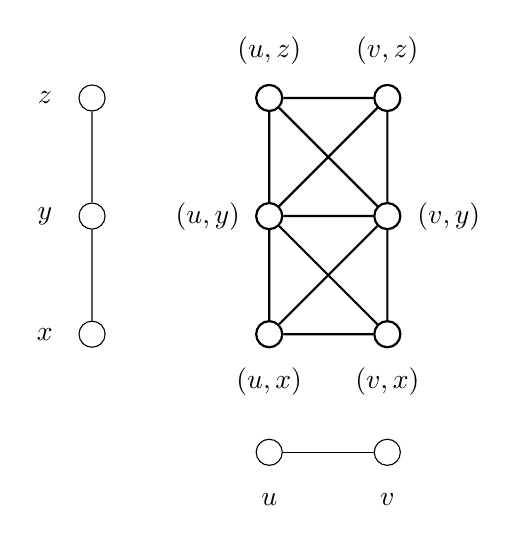
\begin{tikzpicture}[xscale=1.5, yscale=1.5]
                \tikzmath{\o = 0.4;}
                \begin{scope}[every node/.style={circle,draw}]
                \node (u) at (1,0) {};
                \node (v) at (2,0) {};
                
                \node (x) at (-0.5,1) {};
                \node (y) at (-0.5,2) {};
                \node (z) at (-0.5,3) {};
                \end{scope}
                
                \node at (1, -\o) {$u$};
                \node at (2, -\o) {$v$};
                
                \node at (-0.5-\o, 1) {$x$};
                \node at (-0.5-\o, 2) {$y$};
                \node at (-0.5-\o, 3) {$z$};
                
                \path[-,draw]
                (u) edge (v)
                (x) edge (y)
                (y) edge (z);
                
                \begin{scope}[every node/.style={circle,thick,draw}]
                \node (ux) at (1,1) {};
                \node (uy) at (1,2) {};
                \node (uz) at (1,3) {};
                \node (vx) at (2,1) {};
                \node (vy) at (2,2) {};
                \node (vz) at (2,3) {};
                \end{scope}
                
                \node at (1, 1-\o) {$(u,x)$};
                \node at (2, 1-\o) {$(v,x)$};
                \node at (1-1.3*\o, 2) {$(u,y)$};
                \node at (2+1.3*\o, 2) {$(v,y)$};
                \node at (1, 3+\o) {$(u,z)$};
                \node at (2, 3+\o) {$(v,z)$};
                
                \path[-,draw,thick]
                (ux) edge (uy)
                (uy) edge (uz)
                (vx) edge (vy)
                (vy) edge (vz)
                (ux) edge (vx)
                (uy) edge (vy)
                (uz) edge (vz)
                (ux) edge (vy)
                (uy) edge (vx)
                (uy) edge (vz)
                (uz) edge (vy);
            \end{tikzpicture}
        \end{subfigure}
        \caption{Na sliki sta prikazana kartezični produkt $P_2 \boxempty P_3$ (levo) in $P_2 \boxtimes P_3$ (desno). Kartezični produkt označujemo z $\boxempty$, krepki produkt pa z $\boxtimes$ ravno zaradi rezultata teh dveh produktov poti $P_2$ same s seboj.}
        \label{fig:produkta-poti}
    \end{figure}
    
    Pri obeh produktih opazimo, da kot inducirani podgrafi za ustrezno izbrano podmnožico vozlišč nastopajo 3 (ravno $|P_3|$) kopije grafa $P_2$ in 2 (ravno $|P_2|$) kopiji grafa $P_3$.
    
    Na spodnjih slikah je prikazan še primer kartezičnega in krepkega produkta cikla in poti na $n$ vozliščih, natančneje $C_4 \boxempty P_n$ na sliki~\ref{fig:kartez-produkt-cikel-pot} in $C_4 \boxtimes P_n$ na sliki~\ref{fig:krep-produkt-cikel-pot}.
    \begin{figure}[h]
        \centering
        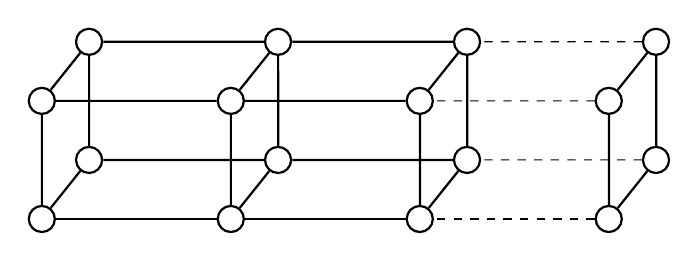
\begin{tikzpicture}[xscale=1.2,yscale=1.5]
        \foreach \i in {1,...,4}
        {
            \begin{scope}[every node/.style={circle,thick,draw}]
                \node (u\i) at (2*\i,0) {};
                \node (v\i) at (2*\i,1) {};
                \node (x\i) at (2*\i+0.5,0.5) {};
                \node (y\i) at (2*\i+0.5,1.5) {};
            \end{scope}
            
            \path[-,thick,draw]
            (u\i) edge (v\i)
            (x\i) edge (y\i)
            (u\i) edge (x\i)
            (v\i) edge (y\i);
            \ifthenelse{\i=1}{}{
                \tikzmath{\im = \i-1;}
                \ifthenelse{\NOT \i=4}{
                    \path[-,thick,draw]
                    (u\i) edge (u\im)
                    (v\i) edge (v\im)
                    (x\i) edge (x\im)
                    (y\i) edge (y\im);
                }{
                    \path[dashed,draw]
                    (u\i) edge (u\im)
                    (v\i) edge (v\im)
                    (x\i) edge (x\im)
                    (y\i) edge (y\im);
                }
            }
        }
        \end{tikzpicture}
        \caption{Prikazan je kartezični produkt $C_4 \boxempty P_n$.}
        \label{fig:kartez-produkt-cikel-pot}
    \end{figure}
    
    \begin{figure}[h]
        \centering
        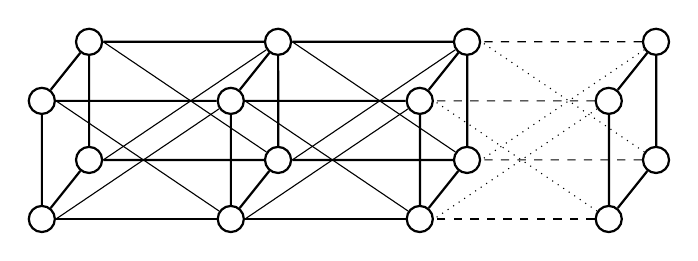
\begin{tikzpicture}[xscale=1.2,yscale=1.5]
        \foreach \i in {1,...,4}
        {
            \begin{scope}[every node/.style={circle,thick,draw}]
            \node (u\i) at (2*\i,0) {};
            \node (v\i) at (2*\i,1) {};
            \node (x\i) at (2*\i+0.5,0.5) {};
            \node (y\i) at (2*\i+0.5,1.5) {};
            \end{scope}
            
            \path[-,thick,draw]
            (u\i) edge (v\i)
            (x\i) edge (y\i)
            (u\i) edge (x\i)
            (v\i) edge (y\i);
            \ifthenelse{\i=1}{}{
                \tikzmath{\im = \i-1;}
                \ifthenelse{\NOT \i=4}{
                    \path[-,thick,draw]
                    (u\i) edge (u\im)
                    (v\i) edge (v\im)
                    (x\i) edge (x\im)
                    (y\i) edge (y\im);
                    \path[-,draw]
                    (u\i) edge (v\im)
                    (v\i) edge (u\im)
                    (x\i) edge (y\im)
                    (y\i) edge (x\im);
                }{
                \path[dashed,draw]
                (u\i) edge (u\im)
                (v\i) edge (v\im)
                (x\i) edge (x\im)
                (y\i) edge (y\im);
                \path[dotted,draw]
                (u\i) edge (v\im)
                (v\i) edge (u\im)
                (x\i) edge (y\im)
                (y\i) edge (x\im);
                
                }
            }
        }
        \end{tikzpicture}
        \caption{Prikazan je krepki produkt $C_4 \boxtimes P_n$.}
        \label{fig:krep-produkt-cikel-pot}
    \end{figure}
\end{primer}

Iz zgornjih definicij in primerov lahko vidimo, da sta tako kartezični kot tudi krepki produkt komutativna produkta, do izomorfnosti grafov natančno. Poglejmo si še en grafovski produkt, za katerega pa komutativnost v splošnem ne velja.

\begin{definicija}
    \emph{Korona} grafov $G$ in $H$, označimo jo z $G \circ H$, je graf velikosti $|G||H| + |G|$, ki ga sestavimo tako, da vzamemo eno kopijo $G$ in $|G|$ kopij grafa $H$, vsa vozlišča $i$-te kopije $H$ pa povežemo z $i$-tim vozliščem v kopiji grafa $G$.
\end{definicija}
Na spodnji sliki~\ref{fig:korona-poti-cikla} sta prikazani koroni $C_5 \circ P_2$ in $P_2 \circ C_5$.

\begin{figure}[h]
    \begin{subfigure}{0.33\textwidth}
        \centering
        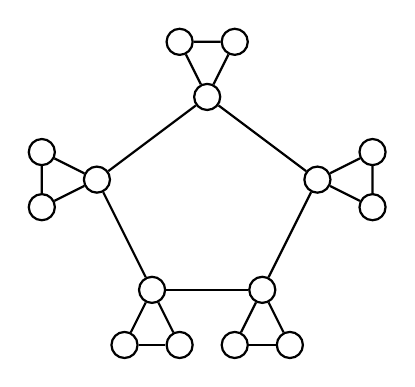
\begin{tikzpicture}[scale=0.7]
        \begin{scope}[every node/.style={circle,thick,draw}]
        \node (1) at (0,0) {};
        \node (2) at (2,0) {};
        \node (3) at (3,2) {};
        \node (4) at (1,3.5) {};
        \node (5) at (-1,2) {};
        
        \node (u1) at ([shift=({-0.5,-1})]1) {};
        \node (v1) at ([shift=({0.5,-1})]1) {};
        
        \node (u2) at ([shift=({-0.5,-1})]2) {};
        \node (v2) at ([shift=({0.5,-1})]2) {};
        
        \node (u3) at ([shift=({1,-0.5})]3) {};
        \node (v3) at ([shift=({1,0.5})]3) {};
        
        \node (u4) at ([shift=({-0.5,1})]4) {};
        \node (v4) at ([shift=({0.5,1})]4) {};
        
        \node (u5) at ([shift=({-1,-0.5})]5) {};
        \node (v5) at ([shift=({-1,0.5})]5) {};
        \end{scope}
        
        \path[-,thick,draw]
        (1) edge (2)
        (2) edge (3)
        (3) edge (4)
        (4) edge (5)
        (5) edge (1);
        
        \foreach \i in {1,...,5}
        {
            \path[-,thick,draw]
            (u\i) edge (v\i)
            (u\i) edge (\i)
            (v\i) edge (\i);
        }
        \end{tikzpicture}
    \end{subfigure}
    \begin{subfigure}{0.66\textwidth}
        \centering
        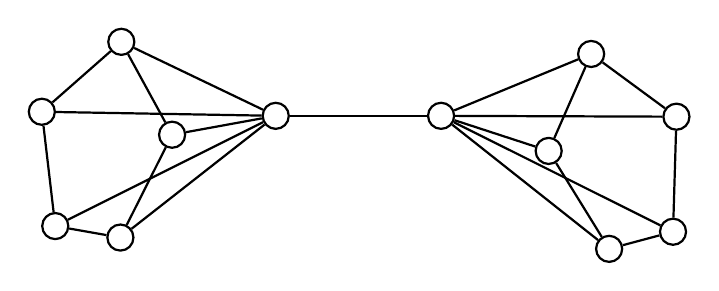
\begin{tikzpicture}[scale=0.7]
        \begin{scope}[every node/.style={circle,thick,draw}, rotate=-10, xscale=0.6]
        \node (1) at (0,0) {};
        \node (2) at (2,0) {};
        \node (3) at (3,2) {};
        \node (4) at (1,3.5) {};
        \node (5) at (-1,2) {};
        \end{scope}
        
        \begin{scope}[every node/.style={circle,thick,draw}, rotate=15, xscale=0.6, shift={(16,-3)}]
        \node (6) at (0,0) {};
        \node (7) at (2,0) {};
        \node (8) at (3,2) {};
        \node (9) at (1,3.5) {};
        \node (10) at (-1,2) {};
        \end{scope}
        
        \begin{scope}[every node/.style={circle,thick,draw}]
         \node (v1) at (4,2) {};
         \node (v2) at (7,2) {};
        \end{scope}
        
        \path[-,thick,draw]
        (1) edge (2)
        (2) edge (3)
        (3) edge (4)
        (4) edge (5)
        (5) edge (1)
        (6) edge (7)
        (7) edge (8)
        (8) edge (9)
        (9) edge (10)
        (10) edge (6)
        (v1) edge (v2);
        
        \foreach \i in {1,...,5} {
            \path[-,thick,draw]
            (\i) edge (v1);
        }
        \foreach \i in {6,...,10} {
            \path[-,thick,draw]
            (\i) edge (v2);
        }
        \end{tikzpicture}
    \end{subfigure}
    \caption{Na sliki sta prikazana korona $C_5 \circ P_2$ (levo) in $P_2 \circ C_5$ (desno). Že iz velikosti lahko vidimo, da grafa nista izomorfna.}
    \label{fig:korona-poti-cikla}
\end{figure}

\subsection{Ničelna prisila}

Poglejmo si osnovno definicijo pojmov, ki so temelji tega dela, in jih demonstrirajmo na preprostih primerih.

\begin{definicija}
    \emph{Množica ničelne prisile} $Z$ grafa $G$ je podmnožica vozlišč tega grafa, takšna, da velja: če na začetku s črno barvo pobarvamo vsa vozlišča iz $Z$, potem pa sledimo pravilu, da vsako črno vozlišče $u$ z natanko enim belim sosedom $v$ prisili vozlišče $v$, da spremeni barvo v črno, in postopek ponavljamo, dokler se še dogajajo kakšne spremembe, morajo biti po koncu postopka vsa vozlišča grafa $G$ pobarvana črno.
\end{definicija}

\begin{primer}
    Za graf na sliki~\ref{fig:osnovni-primer-prisile} je množica ničelne prisile na primer $Z = \{ 1, 5\}$. 
    \begin{figure}[h]
        \centering
        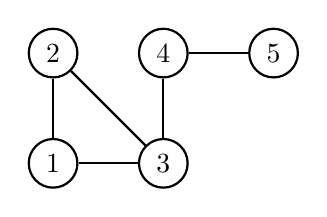
\begin{tikzpicture}[scale=0.7]
        \begin{scope}[every node/.style={circle,thick,draw}]
        \node (1) at (0,0) {1};
        \node (2) at (0,2) {2};
        \node (3) at (2,0) {3};
        \node (4) at (2,2) {4};
        \node (5) at (4,2) {5};
        \end{scope}
        
        \path[-,thick,draw]
        (1) edge (2)
        (2) edge (3)
        (1) edge (3)
        (3) edge (4)
        (4) edge (5);
        
        \end{tikzpicture}
        \caption{Ena izmed petih možnih množic ničelne prisile velikosti~2 grafa na sliki je množica $Z =\{1,5\}$.}
        \label{fig:osnovni-primer-prisile}
    \end{figure}
    Pravzaprav od podmnožic vozlišč velikosti~2 zadostujejo tiste, ki vsebujejo vozlišče~1 ali vozlišče~2 ter hkrati vozlišče~3 ali vozlišče~5, pa tudi podmnožica, ki vsebuje tako vozlišče~1 kot vozlišče~2. (Če se virus začne širiti iz trikotnika, potem morata biti pobarvani vsaj dve izmed vozlišč trikotnika, če pa se začne širiti iz vozlišča~5, ki je stopnje 1, mora biti pobarvano vsaj še eno vozlišče trikotnika (1 ali 2), da bo vozlišče~3 lahko okužilo zadnje neokuženo vozlišče trikotnika.) Vse možne množice ničelne prisile velikosti~2 so torej:
    \[ Z_1 = \{ 1, 2\}, Z_2 = \{ 1, 3\},\ Z_3 = \{ 1, 5\},\ Z_4 = \{ 2, 3\},\ Z_5 = \{2, 5\}. \]
    Če gledamo podmnožice vozlišč velikosti~3, pa so množice ničelne prisile vse, razen tista, ki ne vsebuje ne vozlišča~1 ne vozlišča~2, torej množica $\{3, 4, 5\}$. Množice ničelne prisile velikosti 4 so očitno vse možne podmnožice vozlišč velikosti 4.
\end{primer}

Zanima nas, kakšna je najmanjša možna množica vozlišč, ki jo moramo vzeti, da bo po končanem postopku barvanja celoten graf pobarvan črno. 

\begin{definicija}
    \emph{Število ničelne prisile} $Z(G)$ grafa $G$ je definirano kot velikost najmanjše množice ničelne prisile grafa $G$, oziroma
    \[ Z(G) = \min \{|Z| \mid Z \subseteq V(G) \text{ množica ničelne prisile grafa } G \}. \]
\end{definicija}

Hitro vidimo, da je število ničelne prisile dobro definirano, saj lahko za poljuben graf vedno vzamemo vsa vozlišča, razen enega, in s tem dobimo množico ničelne prisile. Velja torej
\[ Z(G) \leq |G| - 1. \]
Po drugi strani seveda velja tudi, da moramo za zadostitev definicije vedno imeti vsaj eno vozlišče, da lahko govorimo o množici ničelne prisile, očitno velja
\[ Z(G)  \geq 1. \]
Hitro lahko postavimo boljšo očitno spodnjo mejo. Če imamo graf z najmanjšo stopnjo vozlišča $\delta$, mora biti velikost množice ničelne prisile $|Z|$ vsaj $\delta$. V nasprotnem primeru, če bi torej na začetku pobarvali $\delta - 1$ vozlišč ali manj, bi imelo vsako od pobarvanih vozlišč stopnjo vsaj $\delta$, torej bi imelo vsako od pobarvanih vozlišč $u$ vsaj $\delta - (\delta - 1 - 1) = 2$ nepobarvana soseda (ker je $u$ eno izmed pobarvanih vozlišč in ni samo svoj sosed) in se proces širjenja barve sploh ne bi mogel začeti. Velja torej spodnja meja
\[ Z(G) \geq \delta.  \]
Ta spodnja meja je tesna za splošen graf $G$ brez dodatnih omejitev: če vzamemo primer poti $P_n$, ki ima $\delta = 1$, vidimo, da je $Z(G)$ prav tako enak 1 (pobarvamo eno od krajišč poti), torej $Z(P_n) = \delta(P_n).$

Smiselno je vprašati se, ali je ob neki začetni množici pobarvanih vozlišč $Z$, ki ni nujno množica ničelne prisile, končen rezultat postopka širjenja barve vedno enaka množica neodvisno od vrstnega reda spreminjanja barve. Pokažimo:
\begin{trditev}
    Končna množica pobarvanih vozlišč za neko začetno množico $Z$ je vedno ista, ne glede na vrstni red sprememb barv. 
\end{trditev}
\begin{proof}
    Pokažimo, da vozlišče, ki postane črno za nek vrstni red sprememb barv, lahko vedno postane črno, s pomočjo indukcije na število sprememb barv, ki so potrebne, da pobarvamo vozlišče~\cite[str.~1633]{aim2008minimumrank}. 
    
    Fiksirajmo $Z$. Recimo, da za počrnitev vozlišča $u$ potrebujemo 1 spremembo barve. To pomeni, da je $u$ edini nepobarvan sosed enega izmed vozlišč v $Z$ (sprememba barve, ki jo potrebujemo, je ravno barva vozlišča $u$). Ne glede na to, v kakšnem vrstnem redu spreminjamo barve vozlišč, bo $u$ še vedno edini nepobarvan sosed enega izmed vozlišč v $Z$ in bo nekoč pobarvan.
    
    Sedaj naj naša trditev velja za vozlišča, ki potrebujejo $n-1$ sprememb barv, da postanejo črna. Recimo, da za vozlišče $u$ potrebujemo $n$ sprememb barv. To pomeni, da obstaja sosed $v$, ki potrebuje $n-1$ sprememb barv, da počrni, pri čemer bo vozlišče $u$ po tem edini nepobarvan sosed vozlišča $v$. Ker smo predpostavili, da trditev drži za vozlišča, ki potrebujejo $n-1$ sprememb, torej velja, da bo vozlišče $v$ postalo črno neodvisno od vrstnega reda sprememb. Po nekem vrstnem redu sprememb imamo torej črno vozlišče $v$, katerega edini nepobarvan sosed je $u$, ki bo torej (nekoč) postal črn. Torej tudi za vozlišče $u$ velja, da bo postalo pobarvano neodvisno od vrstnega reda sprememb, in indukcija je zaključena.
\end{proof}

Poglejmo si še, zakaj temu pojmu rečemo ``ničelna prisila''. Najprej definirajmo graf $\G(A)$ simetrične matrike $A$ velikosti $n$ nad poljem~$\F$ (pišemo $A \in Sym_n(\F)$):
\[ V(\G(A)) = \{1, \ldots n\},\ E(\G(A)) = \{\{i,j\} \mid a_{ij} \neq 0, 1 \leq i < j \leq n \}. \]
\begin{primer}
    Graf, ki pripada matriki \[ A = \begin{bmatrix*}[r]
    5 & -2 & 3 & 0 & 0 \\
    -2 & 13 & 6.9 & 0 & 0 \\
    3 & 6.9 & 0 & 7 & 0 \\
    0 & 0 & 7 & -1.1 & 1 \\
    0 & 0 & 0 & 1 & 0 \\
    \end{bmatrix*},\] je prikazan na sliki~\ref{fig:osnovni-primer-prisile}.
\end{primer}
Sedaj lahko definiramo množico vseh (simetričnih) matrik grafa $G$ nad poljem~$\F$:
\[ S(\F, G) = \{A \in Sym_n(\F) \mid \G(A) = G \}. \]
Ideja za imenom ničelne prisile je sledeča. Črna vozlišča predstavljajo tiste koordinate v vektorju, za katere zahtevamo, da so enake nič, bela vozlišča pa so tiste koordinate, za katere (še) ni nobene zahteve. Sprememba barve $i$-tega vozlišča iz bele v črno pomeni, da mora $i$-ta koordinata biti nič pri predpostavki, da so vse ostale koordinate, katerih vozlišča so trenutno črna, enake nič in je vektor v jedru matrike grafa $G$. Brez dokaza navedimo
\begin{trditev}[{\cite[trditev 2.3]{aim2008minimumrank}}]
    Imejmo množico ničelne prisile $Z$ grafa $G$ in matriko $A \in S(\F, G)$ grafa $G$ nad poljem $\F$. Naj bo vektor $x$ v jedru matrike $A$. Če so vse koordinate, ki pripadajo vozliščem iz $Z$, enake 0, potem je $x = 0$.
\end{trditev}
\section{Osnovni rezultati}

\subsection{Poti}

\subsection{Cikli}

\subsection{Polni grafi}

\subsection{Zvezde}

\subsection{Kolesa}

\subsection{Trikotniki}

\section{Ekstremni primeri}

\section{Ničelna prisila produktov grafov}


% Literatura:
% Primer navajanja na http://www.fmf.uni-lj.si/storage/24240/LiteraturaM.pdf,
% ampak bi moral stil poskrbeti za vse. Reference se uredijo po abecedi.
% Če nobena izbira izmed @book, @atricle,... ni ok, potem se lahko vse napiše v
% @misc pod note={} in deluje tako kot normalen LaTeX.
% Komentar v bib datoteki se naredi samo s parom { }
% Za urejanje literature avtor priporoča program Jabref, ki zna tudi avtomatsko
% okrajšati imena revij. Za pravilno sortiranje vnosov brez avtorja, uporabite
% polje key={ }, kot v primeru.
% V primeru napak ustvarite issue na GitHubu ali pišite na jure.slak@fmf.uni-lj.si.
\cleardoublepage                           % na desni strani
\phantomsection                            % da prav delujejo hiperlinki
\addcontentsline{toc}{section}{\bibname}   % dodajmo v kazalo
\bibliographystyle{fmf-sl}                 % uporabljen stil je v datoteki fmf-sl.bst, na voljo tudi angleška verzija
\bibliography{\literatura}                 % literatura je v datoteki, definirani na začetku

% Za stvarno kazalo
%\cleardoublepage                           % na desni strani
%\phantomsection                            % da prav delujejo hiperlinki
%\addcontentsline{toc}{section}{\indexname} % dodajmo v kazalo
%\printindex

\end{document}
